
This chapter provides an overview of fundamental concepts related to the work
and a running example to guide the presentation of the evaluation method in
later sections.  We assume the reader is familiar with software product
lines~\cite{clements_software_2002,pohl_software_2010} and discrete-time Markov
chains~\cite{baier_principles_2008}.


%%%%%%%%%%%%%%%%%%%%%%%%%%%%%%%%%%%%%%%%%%%%%%%%%%%%%%%%%%%%%%%%%%%%%%%%%%%%%%%%
%% MODEL CHECKING 
%%%%%%%%%%%%%%%%%%%%%%%%%%%%%%%%%%%%%%%%%%%%%%%%%%%%%%%%%%%%%%%%%%%%%%%%%%%%%%%%
\section{Model Checking \label{sec:modelChecking}}

Model checking is a verification technique that systematically explores the
possible states in a formal model of the system in order to find out whether it
a given property is satisfied or not by software\cite{baier_principles_2008}.

Such analysis is realized by an automated evaluation method that performs an
exhaustive search over the state space that represent the software's behavior.
The fulfillment of the  property under investigation is formally verified in
each reachable state such the model checker answers \emph{yes} in case it is
satisfied or \emph{no}, otherwise. For last case, the model checker also
presents a counter-example to indicate how the unexpected result can be reached
again\cite{baier_principles_2008}. 
The models considered and verified by model checkinng techniques are usually
finite-state automata. In such models, each state represents the conditions
reached by the software after each actions it takes, and such actions are
associated to every transition between two states. 

In special, model checking techniques are used to evaluate probabilistic
properties of software. Markov Chain is a modeling notation usually employed for
representing such probabilistic behavior, which considers the probability of
transitioning from a state to another depends uniquely from the current state.
Discrete-Time Markov Chain (DTMC) is a kind of Markov Chain where each
transition taken represents that a time unity has deccurred.  Parametric Markov
Chains (PMC) extend DTMCs with the ability to represent variable transition
probabilities. Whereas probabilistic choices are fixed at modeling time and
represent possible behavior that is unknown until run time, variable transitions
represent behavior that is unknown already at modeling time. These variable
transition probabilities is useful to represent probabilities in a model whose
values varies according to software or the context\cite{ghezzi_model-based_2013,
rodrigues_modeling_2015}. 



%%%%%%%%%%%%%%%%%%%%%%%%%%%%%%%%%%%%%%%%
%% Software Reliability 
%%%%%%%%%%%%%%%%%%%%%%%%%%%%%%%%%%%%%%%%
\subsection{Software Reliability \label{subsec:softwareReliability}}

Probabilistic verification techniques have been used in the past to substitute
the concept of absolute correctness by bounds on the probability that certain
behavior may occur~\cite{grunske_specification_2008}.  Based on probabilistic
models, it is possible to specify probabilistic system behavior due to, e.g.,
intrinsically unreliable hardware components and environmental characteristics.
Reliability can be defined as a probabilistic existence
property~\cite{grunske_specification_2008}, in the sense that it is given by the
probability of eventually reaching some set of \emph{success} states in a
probabilistic behavioral model of a system. In the setting of this work success
is defined to mean that all tasks of interest have been accomplished by the software as
intended.

Discrete-time Markov Chain (DTMC) is a well-known formalism to model such
probabilistic behavior.  In a DTMC, the reachability probability is defined as
the sum of probabilities for each possible path that starts in an \emph{initial}
state and ends in a state belonging to the set of target states
\cite{baier_principles_2008}.  Thus, to compute reliability the states
considered successfull are labelled with the atom \emph{``success''} and to
compute the reachability probability of success states, expressed as
$P_{=?}[\diamondsuit \mathit{``success"}]$ in the query language of the PARAM
model checker \cite{Hahn_param_2010}.
% define the reachability probability in a probabilistic model $\mathcal{M}$ is
% given by \[ Pr^{\mathcal{M}}(\diamondsuit B) = \sum_{s_0 \dots s_n \in
% Paths_{fin}(\mathcal{M})} l_{init}(s_0) \cdot P(s_0 \dots s_n) \] which,
% intuitively, is the sum of probabilities for all paths from the initial state
% $s_0$ leading to the state $s_n$ where the property $B$ holds, and each path's
% probability is given by the product of all reliabilities values along the
% path.  In the case the states considered successfull are labeled with the
% atomic proposition \emph{``success''}, the problem of finding a reliability
% value for a DTMC $\mathcal{M}$ can be expressed in Probabilistic Computation
% Tree Logic (PCTL)~\cite{baier_principles_2008} as the formula
% $Pr^{\mathcal{M}}(\diamondsuit \mathit{success})$. 




%%%%%%%%%%%%%%%%%%%%%%%%%%%%%%%%%%%%%%%%%%%%%%%%%%%%%%%%%%%%%%%%%%%%%%%%%%%%%%%%
%% SOFTWARE PRODUCT LINE 
%%%%%%%%%%%%%%%%%%%%%%%%%%%%%%%%%%%%%%%%%%%%%%%%%%%%%%%%%%%%%%%%%%%%%%%%%%%%%%%%
\section{Software Product Line \label{sec:softwareProductLine}}

 Software product lines have gained momentum in the software industry as they
 provide a mass customization by building individual products (tailored for the
 customer's requirements) from a set of reusable parts. Since a software product
 line is defined aiming to reuse software parts to build a product, its usage
 brings the benefits of improved quality of the products it creates meanwhile it
 reduces the development costs and time to market. A Software Product Line is defined as a set of software-intensive systems that share
a common, managed set of features satisfying the specific needs of a particular market
segment or mission and that are developed from a common set of core assets in a prescribed
way\cite{clements_software_2002}. 


The main element in the software product-line engineering to manage the
variability which means having the ability to change or customize a
system\cite{linden_software_2007}. Such variability is usually expressed in terms of features which are used to specify and communicate commonalities and differences of
 the products the software product line can instantiate. They are represented
 graphically by a \textit{feature diagram}, which is a  feature model\cite{czarnecki_generative_2000, kang_1990} depicted
 as a tree that captures the existing dependencies and constraints among the
 features~\cite{apel_feature-oriented_2013}. A product of a product line is
 specified by a valid feature selection that fulfills all feature dependencies.

 A software product line can be build using an annotation-based in case each
 feature is marked accordingly in a common code base, such a product is formed
 by removing codes related to features that do not comprise the product. Also, a
 software product lin can be build by a compositional approach, where each
 feature is implemented in a distinct unit and a product is build by composing
 the elements regarding its feature selection \cite{Kastner_2008}.


In addition,  as all software each product instantiated from a software product line has
 different attributes and characteristics which can be subject to some kind of
 analysis, in special its non-functional requirements. Some analysis techniques
 usually employed to the analysis of usual software are being adapted to analyze
 the products a software product line may instantiate as, for example, type
 checking, model checking, static analysis and theorem
 proving~\cite{thum_classification_2014}. In particular, such task may not be
 feasible in practice~\cite{classen_featured_2013} since  the number of
 products a software product line may instantiate can be huge, sometimes it is
 exponential to the number of features (indeed a software product line may, in
 the worst case,instantiate $2^{|F|}$ products, where $|F|$ denotes the number
 of features.  . 






%%%%%%%%%%%%%%%%%%%%%%%%%%%%%%%%%%%%%%%%
%% Software Product Line Analysis
%%%%%%%%%%%%%%%%%%%%%%%%%%%%%%%%%%%%%%%%
\subsection{ Software Product Line Analysis
	\label{subsec:softwareProductLineAnalysis}}

To analyze the behavior of a product line, it is useful to embed its inherent
variability in such a probabilistic model.  A possible approach is to use
\textit{parametric DTMCs} (PDTMC)~\cite{daws_pmc}, which augment DTMCs with
transition probabilities that can be expressed as variables. A PDTMC is a DTMC
whose probability matrix takes values from a set $X$ of strictly positive
parameters. A PDTMC gives rise to a family of DTMCs by instantiating the formal
parameters to values with an instantiation function $\kappa : \mathbb{Q}_+ \cup
X \mapsto [0,1]$. For a parametric DTMC $D_X$ and an instantiation function
$\kappa, \kappa(D_x)$ denotes the DTMC whose probability matrix is given by
instantiating $D_X$'s formal parameters. For PDTMCs, the reliability analysis
problem can be solved by a \emph{parametric reachability}
algorithm~\cite{HahnHZ10}, which outputs a rational expression (a fraction of
two polynomials) on the same variables as the ones in the input parametric
model.  The idea behind this technique is that evaluating the variables in the
rational expression yields the reliability value of the DTMC that would be
obtained by an equivalent evaluation of the variables in the PDTMC.  However,
this behavioral representation  does not take a variability model (e.g., a
feature model) into account, and thus is not sufficient for representing
\emph{possible} behavior in a product line (i.e, behavior of actual products).

Several analysis techniques have been proposed by researchers for software
product lines, each one taking a particular property into account. To help
researchers and practitioners  understand the similarities and differences among
such techniques,  \citet{thum_classification_2014} propose a classification of
the existing techniques, which is followed in this work. In this context, a
\textit{product-based} reliability analysis operates only on derived
(non-variable) UML behavioral models, whereas the variability model may be used
to generate the models. As it is a brute-force strategy, it is only feasible for
product lines with few products. In contrast, the \textit{family-based} strategy
for reliability analysis operates over variant-rich UML behavioral models and
incorporates the knowledge about valid feature combinations. 
% Often, all implementation artifacts of all features are merged into a single
% virtual product (a.k.a. metaproduct or product simulator) which is used for
% subsequent analysis. 
In a \textit{feature-based}  analysis strategy, the reliability of UML
behavioral models related to each individual feature is analyzed in isolation
from the others, i.e., interactions among features and the knowledge about valid
feature combinations are not incorporated into the analysis. 

Other evaluation strategies may be formed by combining two or more strategies
aforementioned~\cite{thum_classification_2014}. For instance, a
\textit{feature-product} analysis consists  of a feature-based analysis step
followed by a product-based analysis, such the result of the feature-based
analysis is reused by the product-based analysis.  In the context of
reliability, the reliability of UML behavioral models related to each feature is
first evaluated in isolation and then the analysis result is reused when
enumerating and evaluating the reliability of each non-variant UML behavioral
model of the product line. 
In the opposite, the \textit{feature-family based} consists of evaluating each
feature in isolation (ie. a feature-based step) followed by the family-based
evaluation step when each features evaluation's results are reused jointly
with the knowledge about all valid configurations. 

Although other combined evaluation strategies are possible, the aforementioned
strategies suffice as contrast to the hereby proposed strategy.  For more
information regarding the remaining strategies, please refer to
\citet{thum_classification_2014}.








%%%%%%%%%%%%%%%%%%%%%%%%%%%%%%%%%%%%%%%%
%% Feature Discrete-Time Markov Chains 
%%%%%%%%%%%%%%%%%%%%%%%%%%%%%%%%%%%%%%%%
\subsection{Feature Discrete-Time Markov Chains
	\label{subsec:featureDiscreteTimeMarkovChains}}

Featured Discrete-time Markov Chains (FDTMC) \cite{rodrigues_modeling_2015} are
probabilistic models that properly handle product-line variability.  They can be
thought as DTMCs that, instead of transition probabilities, have transition
\emph{probability profiles}.  These profiles are functions $\llbracket
\mathit{FM} \rrbracket \to [0,1]$ that map a configuration to a probability
value, where $\llbracket \mathit{FM} \rrbracket$ denotes the set of valid
configurations of the feature model $\mathit{FM}$.
\citet{rodrigues_modeling_2015} proposed a method to encode an FDTMC as a PDTMC,
enabling its analysis by off-the-shelf parametric model checkers. The present
work leverages the view of \citet{rodrigues_modeling_2015} of FDTMCs
as PDTMCs for the purpose of compositional reliability analysis.

% \citet{rodrigues_modeling_2015} present a way to encode FDTMCs as parametric
% DTMCs, by means of boolean variables that represent features presence or
% absence.  In doing so, they retain the ability to be analyzed by off-the-shelf
% parametric model checkers.  In this work, we also treat FDTMCs as parametric
% DTMCs for practical purposes, but use a different encoding.  Instead of
% representing variability by feature-related parameters, we let variables
% denote arbitrary probabilities and enforce constraints from the feature model
% when valuating them.









%%%%%%%%%%%%%%%%%%%%%%%%%%%%%%%%%%%%%%%%%%%%%%%%%%%%%%%%%%%%%%%%%%%%%%%%%%%%%%%%
%% RUNNING EXAMPLE
%%%%%%%%%%%%%%%%%%%%%%%%%%%%%%%%%%%%%%%%%%%%%%%%%%%%%%%%%%%%%%%%%%%%%%%%%%%%%%%%
\section{Running example \label{sec:runningExample}}

To illustrate the concepts presented throughout this paper, it will be
considered an example of a simple product line within the medical domain, for
which reliability is considered the major requirement~\cite{Hao:2008bs}: the
Body Sensor Network (BSN) product line is a network of connected sensors that
capture vital signs from an individual and send them to a central system to
analyze the collected data and identify critical health
situations~\cite{rodrigues_modeling_2015}.
%Sensors are organized as represented by Figure \ref{fig:BSN}.  The central
%sensor is responsible for optimizing the data collected, filtering redundancy,
%or translating communication protocols. The other sensors are the Accelerometer
%(ACC), Oximeter for blood oxidation and blood oxidation curve (in figure
%represented by SPO2), EKG for heart rate and electrocardiogram curve and TEMP
%for temperature.  This SPL has software components which interpret data
%provided by the sensors and analyze an individual's health situation by
%processing data regarding oxygenation, pulse rate, temperature, position and
%fall occurrences.  Lastly, the BSN has software components for data persistence
%at database or memory. The set of possible configurations to be instantiated
%from this software product line is represented by Figure~\ref{fig:fm}. In such
%feature model, wireless sensors are grouped by the \textit{Sensor} feature, the
%software components for interpreting health information are grouped by
%\textit{SensorInformation} feature and the alternatives for data persistence
%are grouped by \textit{Storage} feature.
This product line has software components that interpret data provided by the
sensors and analyze an individual's health situation, as well as components for
data persistence in a database or memory.  The set of possible configurations
for this product line is defined by its feature model (Figure~\ref{fig:fm}), in
which wireless sensors are grouped by feature \textit{Sensor}, software
components for interpreting health information are grouped by feature
\textit{SensorInformation}, and the alternatives for data persistence are
grouped by feature \textit{Storage}.

% \begin{figure}
% 	\centering
% 	\includegraphics[width=\columnwidth]{./images/body_sensor_network_complete.PNG}
% 	\caption{Body Sensor Network}
% 	\label{fig:BSN}
% \end{figure}

\begin{figure}[ht!]
	\centering
	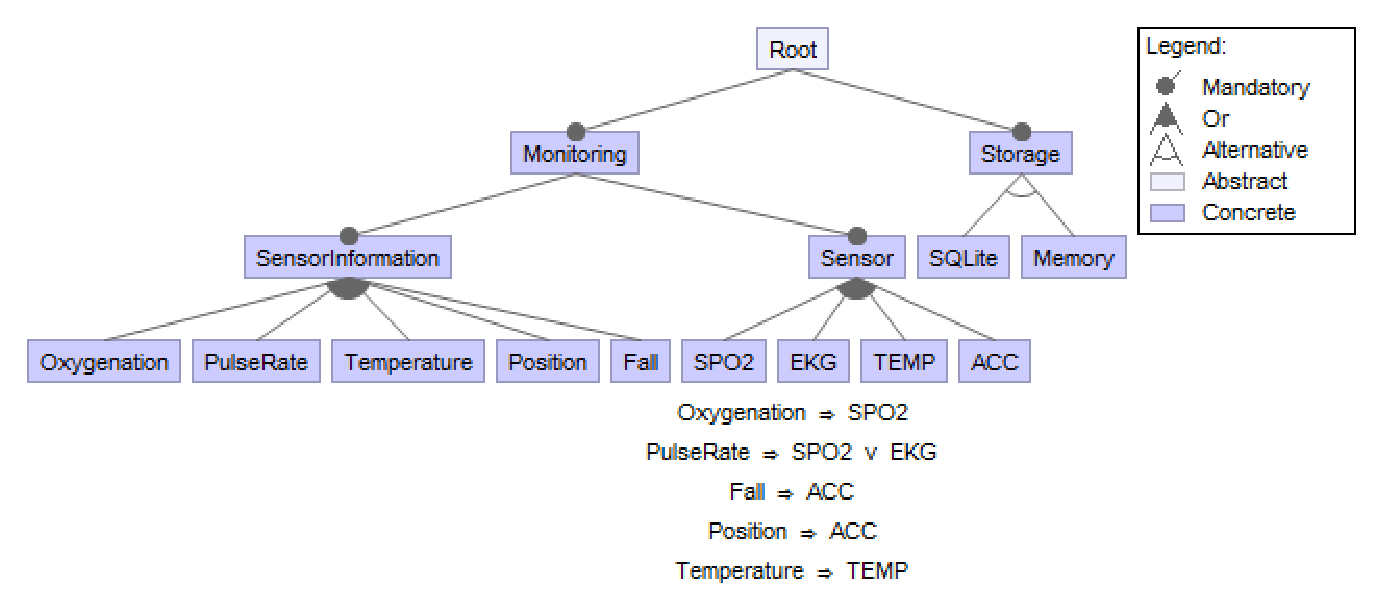
\includegraphics[width=\columnwidth]{./img/fm-full}
	\caption{BSN-SPL Feature Model}
	\label{fig:fm}
\end{figure}


To continuously monitor an individual's health situation, the BSN product line
has a control loop comprised of four activities: capture data coming from
sensors, process information about the health condition, identify health goal
changes, and reconfigure the system if necessary. This control loop represents
the coarse-grained behavior of the BSN product line and it is modeled by the
activity diagram shown in Figure~\ref{fig:bsnControlLoop}, with each activity
being represented in detail by an associated sequence diagram involving the
software components and their behavior. The underlined words in the activities
nodes are the terms by each activity will be referred along this text. Every
product instantiated from the BSN product line executes this control loop and,
whenever the individual's health condition changes and this triggers a
quality-of-service (QoS) goal change, another product is instantiated from this
product line with the desired behavior to reach the desired QoS goal.
By your turn, the behavioral representation provided by sequence diagrams is
considered fine-grained since its elements are able to represent the software
components enrolled in a task execution, the manner how the interactions
between such components happens, in addition to behavioral branches, loops and
variability.  In special, sequence diagrams play the role of representing the
behavioral variability due the software product line where necessary by means
of guard conditions involving the presence of features (a.k.a \emph{presence
conditions} \cite{czarnecki_verifying_2006}).

\begin{figure}[!hbt] 
  \vspace{0.8cm}
  \begin{subfigure}[c]{1.0\textwidth}
  \centering
    %\includegraphics[width=\columnwidth]{img/bsn_AD}
    \tikzset{every node/.style={
             minimum size=6mm, 
             text width=3.5cm,
             font=\itshape,
             align=center,
             draw=none,
             thick, 
             },
         adStart/.style={
             %The shape
             circle,
             text width=0cm,
             draw=black,
             fill = black}, 
         adActiv/.style={
             %The shape
             rounded rectangle,
             draw=black,
             }, 
         adDecis/.style={
             diamond,
             draw=black,
             text width=0cm,
             }, 
         adMerge/.style={
             diamond,
             draw=black,
             text width=0cm,
             } 
}

    \begin{tikzpicture}[transform canvas={scale=0.5}, ultra thick]
  \matrix[row sep=1mm,column sep=5mm, draw=none]{
   \node [adStart](start){}; &
   \node [adActiv](capture){\Large System \underline{captures} vital signal}; &
   \node [adActiv](situation){\Large System identifies \underline{situation}}; &
   \node [adActiv](qosgoal){\Large Compute new \underline{QoS goal}}; & 
   \node [adDecis](decision)[label=below:Was there any QoS goal change?, text width=0.8cm]{}; &
   \node [adActiv](reconfiguration){\Large System \underline{reconfiguration} to achieve new QoS goal}; &
   \node [adMerge](merge)[text width=0.8cm]{}; &
   \node [adStart]{}; \node[circle, minimum width=9mm, text width=0, thick, draw=black](end){}; \\ };
  \draw [-{Latex[width=3mm]}] (start.east) -- (capture.west);
  \draw [-{Latex[width=3mm]}] (capture.east) -- (situation.west);
  \draw [-{Latex[width=3mm]}] (situation.east) -- (qosgoal.west);
  \draw [-{Latex[width=3mm]}] (qosgoal.east) -- (decision.west);
  \draw [-{Latex[width=3mm]}] (reconfiguration.east) -- (merge.west);
  \draw [-{Latex[width=3mm]}] (merge.east) -- (end.west);
  \draw [-{Latex[width=3mm]}] (decision.east) -- (reconfiguration.west) node[midway, sloped, above] {yes};
  \draw [-{Latex[width=3mm]}] (decision.north) -- ++(0,1.2) node[midway, sloped, above] {no} -| (merge.north);
\end{tikzpicture}

    \vspace{0.7cm}
    \caption{Activity Diagram representing the control loop of BSN-SPL}
    \label{fig:bsnControlLoop}
  \end{subfigure}

  \vspace{1cm}
  
  \begin{subfigure}[c]{0.95\columnwidth}
  \centering
    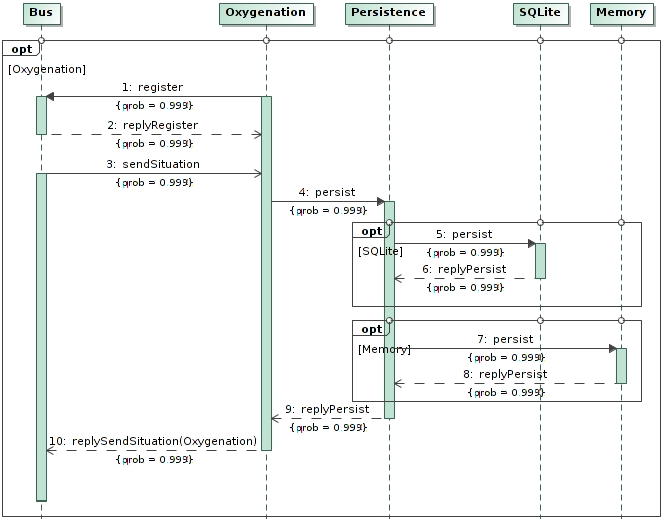
\includegraphics[width=0.7\columnwidth]{img/sd-oxygenation}
    \caption{Sequence diagram (excerpt) associated with the activity
	    \textit{system identifies situation}, for processing and persisting
	    Oxygenation information.} 
    \label{fig:oxygenationSituation} 
  \end{subfigure}
  \label{fig:bsnBehavioralDiagrams}

  \vspace{1cm}
  
  \begin{subfigure}[c]{0.95\columnwidth}
  \centering
    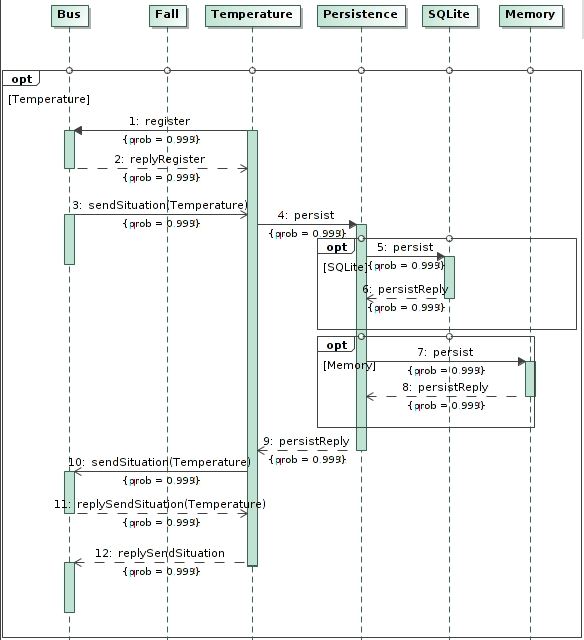
\includegraphics[width=0.7\columnwidth]{img/sd-temperature}
    \caption{Sequence diagram (excerpt) associated with the activity
	    \textit{system identifies situation}, for processing and persisting
	    Temperature information.} 
    \label{fig:temperatureSituation} 
  \end{subfigure}
  \label{fig:bsnBehavioralDiagrams}
  \vspace{12pt} 
  
  \caption{Behavioral diagrams for BSN-SPL}
\end{figure}

For instance, figures~\ref{fig:oxygenationSituation} and \ref{fig:temperatureSituation} presents an excerpt of the
sequence diagram associated with the activity \emph{System identifies
	\underline{situation}}
(Figure~\ref{fig:bsnControlLoop}). This activity consists of processing and
persisting data regarding the individual's health condition, in particular
sensor information, represented by feature \textit{SensorInformation} and its
child features in Figure~\ref{fig:fm}.  Figure~\ref{fig:oxygenationSituation}
depicts the behavior associated with the computation and persistence of the
individual's oxygenation. Such behavior is defined by the messages exchanged
between five software components, whose roles are data processing
($Oxygenation$) and persistence ($Persistence$, $SQLite$ and
$Memory$---$Persistence$ dispatches calls to the concrete persistence engines),
and components for communication and coordination ($Bus$). Each message is named
according to its task and has an associated probability value \texttt{prob} to
represent the reliability of the communication channel between the components
comprising the interaction. The reliability is given by the product of (a) the
probability that the required message arrives at the receiver component and (b)
the receiver component's reliability (i.e., the probability that it performs the
required task without failure).  For the BSN product line, we assume that all
channels have the minimal reliability $0.999$. The same understanding described above applies to the sequence diagram of Figure~\ref{fig:temperatureSituation} since it processes and persists data regarding the individual's temperature.

The guard condition at the top level of the sequence diagram presented in
Figure~\ref{fig:oxygenationSituation} is the atomic proposition
\texttt{Oxygenation}.  This means that the enclosed behavior is associated with
the presence of the \textit{Oxygenation} feature in a given configuration.  This
behavior, in turn, has two variants, according to the chosen mechanism for data
persistence.  The optional fragment whose guard condition is \texttt{SQLite}
models the behavior of persisting data in a database whenever feature $SQLite$
is part of a configuration.  Likewise, the optional fragment associated to the
presence of the feature \textit{Memory} (i.e., the fragment with the
\texttt{Memory} guard) models persistence on secondary memory. In an analogous way the sequence diagram represented in Figure~\ref{fig:temperatureSituation} is associated to the presence of \emph{Oxygenation} feature, since its presence condition is defined by the atom \texttt{Oxygenation}. It also has two variability points for data persistence related to \emph{SQLite} and \emph{Memory} features, respectively.


% To represent this computation in Figure \ref{fig:oxygenationSituation}, depict
% the behavior of handling oxygenation data, which will only be present in
% products having the \textit{Oxygenation} feature as part of its configuration
% (hence the \textit{oxygenation} guard condition).  This task has two further
% variation points, which are guarded by the atomic propositions \textit{sqlite}
% and \textit{memory}.  The constraint that the corresponding features are
% alternative is ensured in the feature model (Figure~\ref{fig:fm}).

Note that the dynamic behavior of the BSN product line does not affect the
method to reliability analysis, since it only considers the execution of tasks
up to reconfiguration (Figure~\ref{fig:bsnControlLoop}).  Moreover, the approach
is entirely based on design-time artifacts.  For a deeper discussion of how the
BSN product line is engineered for reconfiguration and of how the reliability
computation affects this dynamic behavior, please refer to the work by
\citet{ReliableAndMaintainableDSPL}









%% CONCLUSION
%%%%%%%%%%%%%%%%%%%%%%%%%%%%%%%%%%%%%%%%%%%%%%%%%%%%%%%%%%%%%%%%%%%%%%%%%%%%%%%%
\section{Conclusion \label{sec:backgroundConclusion}}

This chapter presented the main topics related to the verification of
probabilistic properties of software product line. The verification of such
properties is indeed important to ensure the desired quality level of the
products a software product line. For such verification the model checking
techniques play a major role but it faces challenges regarding the sizes of the
configuration space and the evaluated models. Nowadays evaluation techniques
propose some improvements in order to reduce the evaluation effort, like the
use of symbolic model checkers, but there is still space for improvements. 

The work hereby presented is, thus, aimed to explore the verification of
probabilistic properties in the context of software product lines, in special,
the reliability property. Such property can be evaluated on probabilistic
models as the reachability measure of states considered successfull. For such
evaluation, the proposed evaluation method seeks to tame the required effort by
employing a \emph{feature-family} strategy that divides the behavioral models
into smaller models, analyze each one in isolation and later reuse their
results to compute the reliability of the whole software product line. 






